\section{Doménový model}\label{sec:domenovyModel}

Pro lepší pochopení dané terminologie je vhodné vytvořit doménový model a popsat jeho entity.
Doménový model je také užitečný jako podklad při návrhu databázového schématu (viz sekce~\ref{sec:databázovéSchéma}).

\subsection{Uživatel}\label{subsec:uživatel}

Entita \texttt{Uživatel} nese uživatelovi přihlašovací informace, email, který bude použit v případě zapomenutého hesla, a čas posledního přihlášení.
Čas posledního přihlášení může být využit například pro odstranění neaktivních účtů.

\subsection{Dokument}\label{subsec:dokument}

Entita \texttt{Dokument} je nositelem informací o dokumentu.
Atribut \texttt{poslední obsah} obsahuje poslední text dokumentu potvrzený serverem, který je posílán nově připojeným klientům.

\subsection{Nastavení dokumentu}\label{subsec:nastaveníDokumentu}

\texttt{Nastavení dokumentu} nese informace o vzhledu a chování editoru pro jednotlivé dokumenty.
Vazba na entitu Uživatel umožňuje vytvoření výchozího nastavení dokumentu pro uživatelem nově vytvořené dokumenty.

\subsection{Operace}\label{subsec:operace}

Entita \texttt{Operace} označuje jednu revizi dokumentu a obsahuje soubor změn, které byli v dokumentu provedeny od předchozí revize.

\subsection{Další entity}\label{subsec:dalšíEntity}

Entita \texttt{Pozvánka} umožňuje uživateli pozvat dalšího uživatele k nahlédnutí, či úpravám dokumentu (podle zvoleného atributu práva).
\texttt{Zpráva} označuje jednu zprávu v komunikačním vlákně dokumentu, z pevné vazby na entitu Uživatel plyne omezení, že zprávu může odeslat pouze přihlášený uživatel.
A poslední entita \texttt{Uživatelský přístup} udržuje informaci o času posledního přístupu uživatele k dokumentu (pro každou dvojici uživatel a dokument existuje nejvýše jedna její instance).

\begin{figure}[ht!]
    \centering
    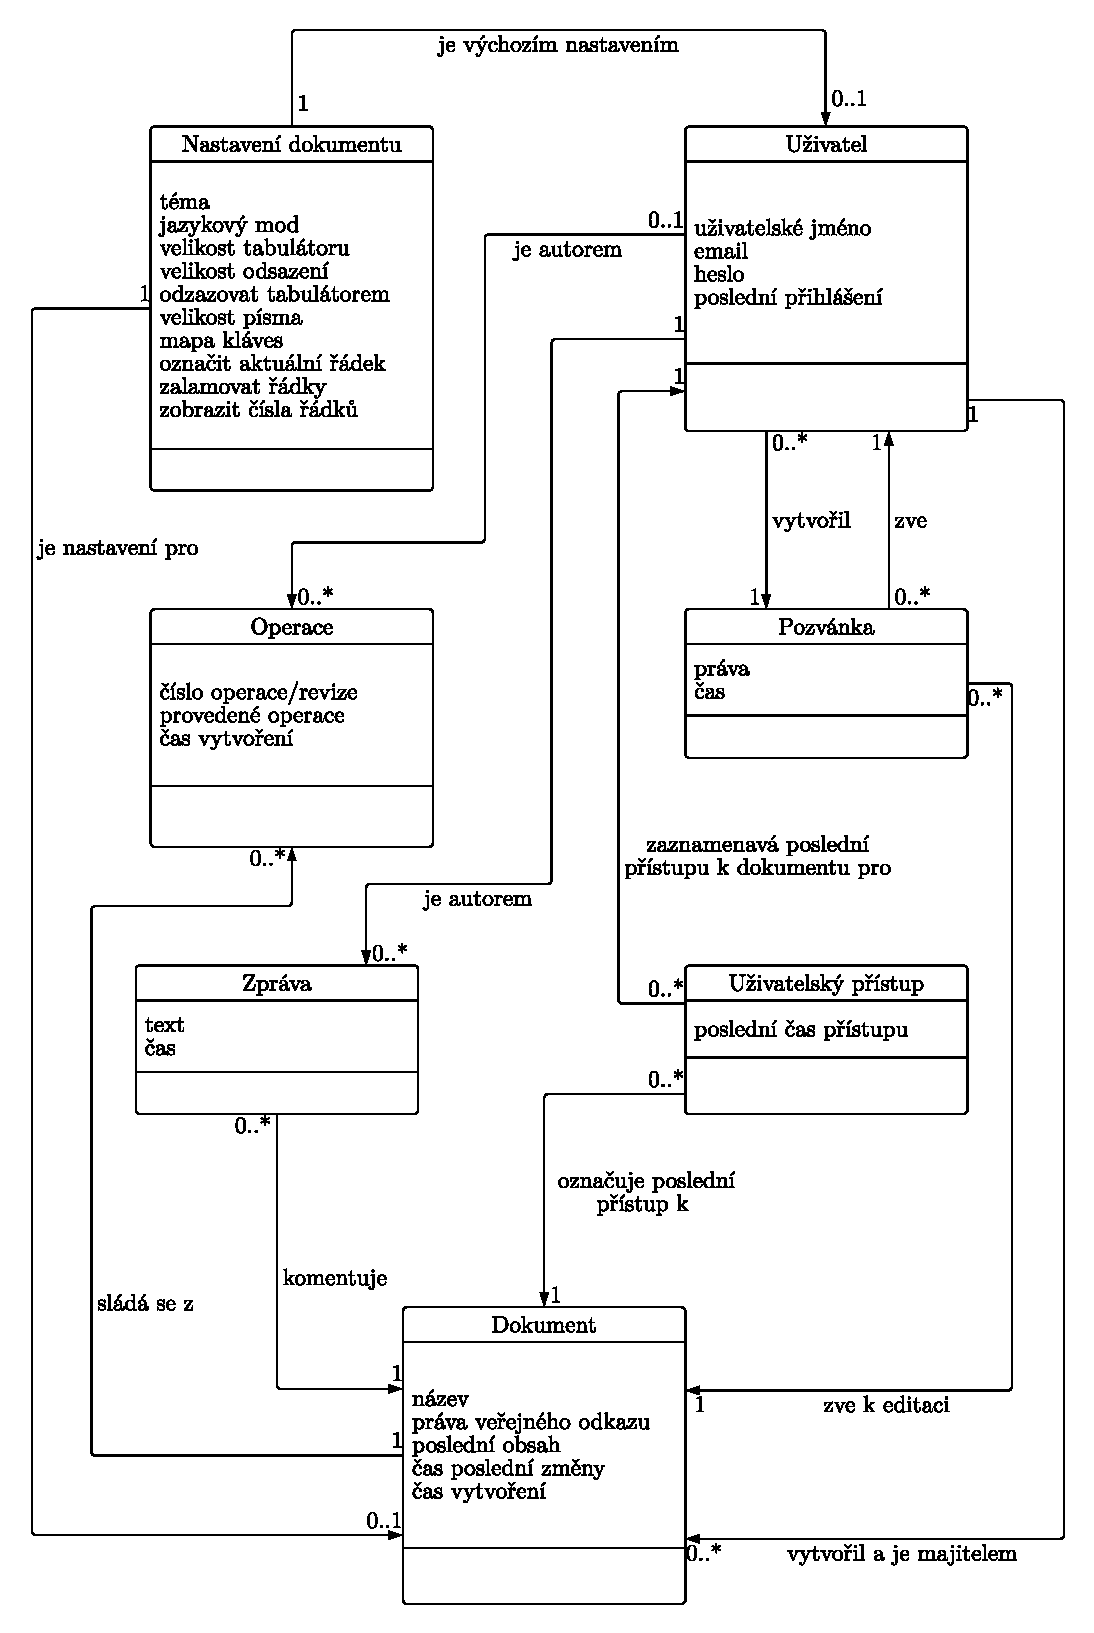
\includegraphics[width=0.9\textwidth]{partials/analyza/domenovy_model-2.pdf}
    \caption{Diagram doménového modelu}\label{fig:domenovy_model}
\end{figure}